\documentclass[spec, och, labwork]{shiza}
% параметр - тип обучения - одно из значений:
%    spec     - специальность
%    bachelor - бакалавриат (по умолчанию)
%    master   - магистратура
% параметр - форма обучения - одно из значений:
%    och   - очное (по умолчанию)
%    zaoch - заочное
% параметр - тип работы - одно из значений:
%    referat    - реферат
%    coursework - курсовая работа (по умолчанию)
%    diploma    - дипломная работа
%    pract      - отчет по практике
% параметр - включение шрифта
%    times    - включение шрифта Times New Roman (если установлен)
%               по умолчанию выключен
\usepackage{subfigure}
\usepackage{tikz,pgfplots}
\pgfplotsset{compat=1.5}
\usepackage{float}

%\usepackage{titlesec}
\setcounter{secnumdepth}{4}
%\titleformat{\paragraph}
%{\normalfont\normalsize}{\theparagraph}{1em}{}
%\titlespacing*{\paragraph}
%{35.5pt}{3.25ex plus 1ex minus .2ex}{1.5ex plus .2ex}

\titleformat{\paragraph}[block]
{\hspace{1.25cm}\normalfont}
{\theparagraph}{1ex}{}
\titlespacing{\paragraph}
{0cm}{2ex plus 1ex minus .2ex}{.4ex plus.2ex}

% --------------------------------------------------------------------------%


\usepackage[T2A]{fontenc}
\usepackage[utf8]{inputenc}
\usepackage{graphicx}
\graphicspath{ {./images/} }
\usepackage{tempora}

\usepackage[sort,compress]{cite}
\usepackage{amsmath}
\usepackage{amssymb}
\usepackage{amsthm}
\usepackage{fancyvrb}
\usepackage{listings}
\usepackage{listingsutf8}
\usepackage{longtable}
\usepackage{array}
\usepackage[english,russian]{babel}

% \usepackage[colorlinks=true]{hyperref}
\usepackage{url}

\usepackage{underscore}
\usepackage{setspace}
\usepackage{indentfirst} 
\usepackage{mathtools}
\usepackage{amsfonts}
\usepackage{enumitem}
\usepackage{tikz}
\usepackage{minted}

\newcommand{\eqdef}{\stackrel {\rm def}{=}}
\newcommand{\specialcell}[2][c]{%
\begin{tabular}[#1]{@{}c@{}}#2\end{tabular}}

\renewcommand\theFancyVerbLine{\small\arabic{FancyVerbLine}}

\newtheorem{lem}{Лемма}

\begin{document}

% Кафедра (в родительном падеже)
\chair{}

% Тема работы
\title{Классификация бинарных отношений и системы замыканий}

% Курс
\course{3}

% Группа
\group{331}

% Факультет (в родительном падеже) (по умолчанию "факультета КНиИТ")
\department{факультета КНиИТ}

% Специальность/направление код - наименование
%\napravlenie{09.03.04 "--- Программная инженерия}
%\napravlenie{010500 "--- Математическое обеспечение и администрирование информационных систем}
%\napravlenie{230100 "--- Информатика и вычислительная техника}
%\napravlenie{231000 "--- Программная инженерия}
\napravlenie{100501 "--- Компьютерная безопасность}

% Для студентки. Для работы студента следующая команда не нужна.
% \studenttitle{Студентки}

% Фамилия, имя, отчество в родительном падеже
\author{Окунькова Сергея Викторовича}

% Заведующий кафедрой
% \chtitle{} % степень, звание
% \chname{}

%Научный руководитель (для реферата преподаватель проверяющий работу)
\satitle{аспирант} %должность, степень, звание
\saname{В. Н. Кутин}

% Руководитель практики от организации (только для практики,
% для остальных типов работ не используется)
% \patitle{к.ф.-м.н.}
% \paname{С.~В.~Миронов}

% Семестр (только для практики, для остальных
% типов работ не используется)
%\term{8}

% Наименование практики (только для практики, для остальных
% типов работ не используется)
%\practtype{преддипломная}

% Продолжительность практики (количество недель) (только для практики,
% для остальных типов работ не используется)
%\duration{4}

% Даты начала и окончания практики (только для практики, для остальных
% типов работ не используется)
%\practStart{30.04.2019}
%\practFinish{27.05.2019}

% Год выполнения отчета
\date{2022}

\maketitle

% Включение нумерации рисунков, формул и таблиц по разделам
% (по умолчанию - нумерация сквозная)
% (допускается оба вида нумерации)
% \secNumbering

%-------------------------------------------------------------------------------------------
\tableofcontents

\section{Постановка задачи}

Цель работы:

Изучение основных свойств бинарных отношений и операций замыкания бинарных отношений.

Порядок выполнения работы:
    \begin{enumerate}
        \item Разобрать основные определения видов бинарных отношений и разработать
        алгоритмы классификации бинарных отношений.
        \item Изучить свойства бинарных отношений и рассмотреть основные системы
        замыкания на множестве бинарных отношений.
        \item Разработать алгоритмы построения основных замыканий бинарных отношений.
    \end{enumerate}

\section{Теоретические сведения по рассмотренным темам с их обоснованием}

\subsection{Определение бинарного отношения:}
        
        Подмножества декартова произведения $A \cdot B$ множеств $A$ и $B$ называются \textbf{бинарными отношениями} между элементами множеств $A, B$ и обозначаются строчными греческими буквами: $\rho, \sigma, \rho_1, \rho_2, ...$. 

        Для бинарного отношения $\rho \subset A \cdot B$ область определения $D_\rho$ и множество значений $E_\rho$ определяется как подмножества соответствующих множеств $A$ и $B$ по следующим формулам:

        \[D_\rho = \left\{ a: (a, b) \in \rho \text{ для некоторого } b \in B \right\}\]
        \[E_\rho = \left\{ b: (a, b) \in \rho \text{ для некоторого } a \in A \right\}\]

\subsection{Свойства бинарных отношений:}

        Бинарное отношени является:

        \begin{enumerate}
            \item \textit{рефлексивным}, если $(a, a) \in \rho$ для любого $a \in A$;
            \item \textit{антирефлексивным}, если $(a, a) \notin \rho$ для любого $a \in A$;
            \item \textit{симметричным}, если $(a, b) \in \rho \Rightarrow (b, a) \in \rho$;
            \item \textit{антисимметричным}, если $(a, b) \in \rho \text{ и } (b, a) \in \rho \Rightarrow a = b$;
            \item \textit{транзитивным}, если $(a, b) \in \rho \text{ и } (b, c) \in \rho \Rightarrow (a, c) \in \rho$
            \item \textit{антитранзитивным}, если $(a, b) \in \rho \text{ и } (b, c) \in \rho \Rightarrow (a, c) \notin \rho$
        \end{enumerate}

\subsection{Классификация бинарных отношений:}

        Классификация бинарных отношений напрямую определяются их свойствами.

        \begin{enumerate}
            \item Рефлексивное транзитивное отношение называется отношением квазипорядка.
            \item Рефлексивное симметричное транзитивное отношение называется отношением эквивалентности.
            \item Рефлексивное антисимметричное транзитивное отношение называется отношением (частичного) порядка.
            \item Антирефлексивное, антисимметричное и транзитивное отношение называется отношением строгого порядка.
        \end{enumerate}

\subsection{Замыкание отношения:}
        
        \textbf{Замыканием отношения} $R$ относительно свойства $P$ называется такое множество $R^*$, что:
        
        \begin{enumerate}
            \item $R \subset R^*$.
            \item $R^*$ обладает свойством $P$.
            \item $R^*$ является подмножеством любого другого отношения, содержащего $R$ и обладающего свойством $P$.
        \end{enumerate}

\section{Результаты работы}

        \subsection{Описание алгоритма классификации бинарных отношений}
            \begin{enumerate}
                \item Чтобы проверить бинарное отношение на рефлексивность достаточно посмотреть на главную
                диагональ матрицы бинарного отношения. Если все ее элементы являются 1, то бинарное отношение
                является рефлексивным, если же все ее элементы 0, та бинарное отношение является антирефлексивным,
                иначе бинарное отношение является не рефлексивным.
                \item Чтобы проверить бинарное отношение на симетричность нужно транспонировать его матрицу и сравнить
                полученную с исходной, если они равны, то отношение симметрично, иначе нужно проверить на антисиметричность:
                если при умножении матрицу бинарного отношения на себя транспонированную на главной диагонали стоят все 0, 
                то бинарное отношение, явлчется антисиметричным, иначе не симетричным.
                \item Чтобы проверить бинарное отношение на транзитивность нужно возвести его матрицу в квадрат и
                сравнить полученную матрицу с исходной, если исходная матрица $\leq$ полученной матрицы, то бинарное
                отношение является транзитивным, иначе следует поэлементно проверить все элементы бинарного отношения
                на выполнение свойства антитранзитивности, если все элементы удовлетворяют свойству антитранзитивности,
                то отношение антитранзитивное, иначе отношение не является транзитивным.
            \end{enumerate}
        \subsection{Описание алгоритмов построения основных замыканий бинарных отношений}
            \begin{enumerate}
                \item Чтобы построить замыкание на рефлексивности нужно дополнить главную диагональ матрицы бинарного
                отношения 1. 
                \item Чтобы построить замыкание на рефлексивности нужно доставить на симетричных позициях матрицы 
                ($a[i][j]$ и $a[j][i]$) 1, если $a[i][j] = 1$.
                \item Чтобы построить замыкание транзитивности нужно дополнить матрицу до отношениия транзитивности, в моей
                реализации это достигается за счет прохождения матрицы 3 циклами и установки значения $a[i][j] = 1$, если
                $a[i][k] = 1 \wedge a[k][j] = 1$.
            \end{enumerate}
    
        \subsection{Коды программ, реализующей рассмотренные алгоритмы}

            \inputminted[fontsize=\small]{python}{../code/lab1.py}
    
        \subsection{Результаты тестирования программ}

        \begin{figure}[H]
            \centering      %размер рисунка       здесь находится название файла рисунка, без указания формата
            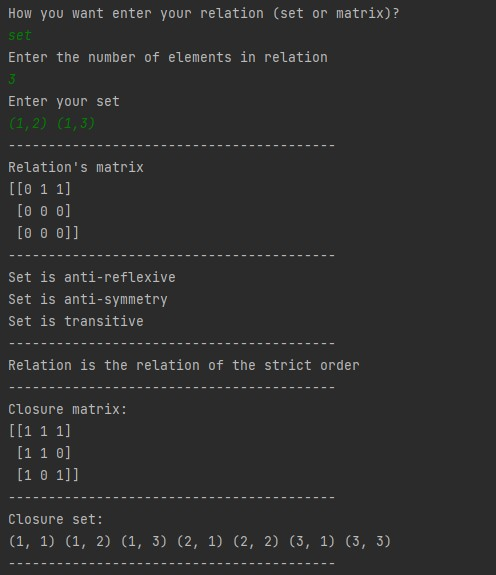
\includegraphics[width=1.\textwidth]{1}
            \caption{Тест 1}
            \label{fig:image1}
        \end{figure}
        
        \begin{figure}[H]
            \centering      %размер рисунка       здесь находится название файла рисунка, без указания формата
            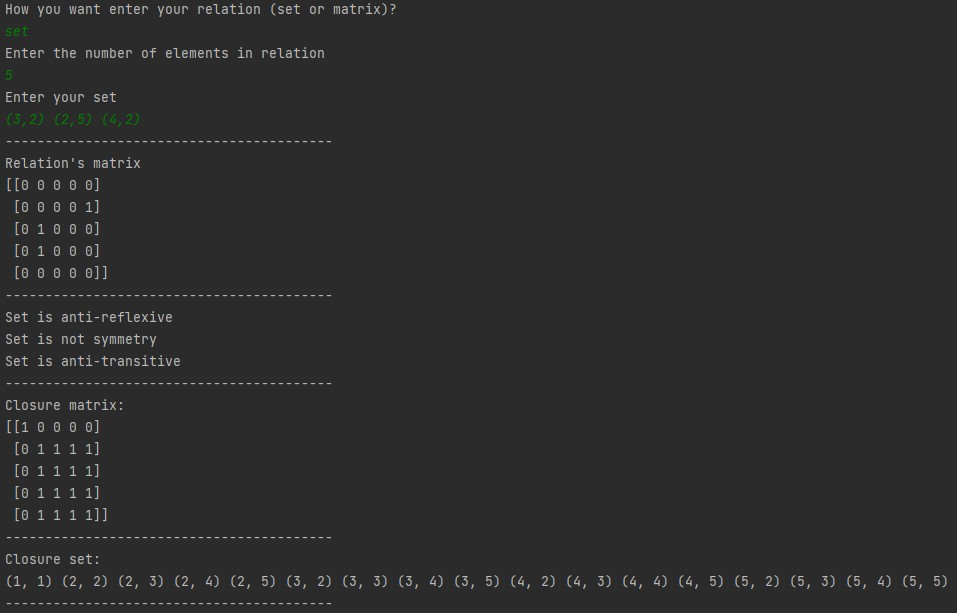
\includegraphics[width=1.\textwidth]{2}
            \caption{Тест 2}
            \label{fig:image1}
        \end{figure}

        \begin{figure}[H]
            \centering      %размер рисунка       здесь находится название файла рисунка, без указания формата
            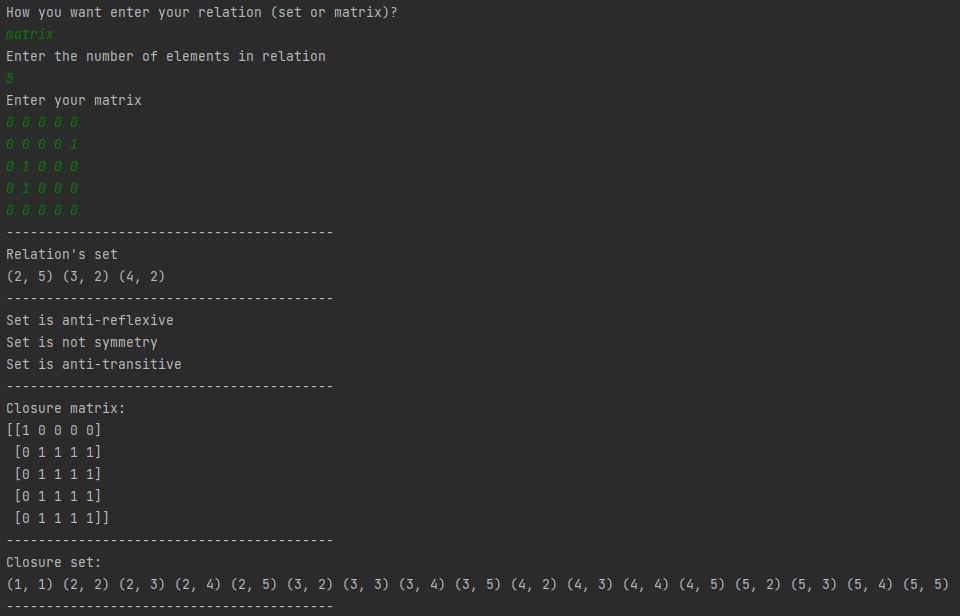
\includegraphics[width=1.\textwidth]{3}
            \caption{Тест 3}
            \label{fig:image1}
        \end{figure}

        \begin{figure}[H]
            \centering      %размер рисунка       здесь находится название файла рисунка, без указания формата
            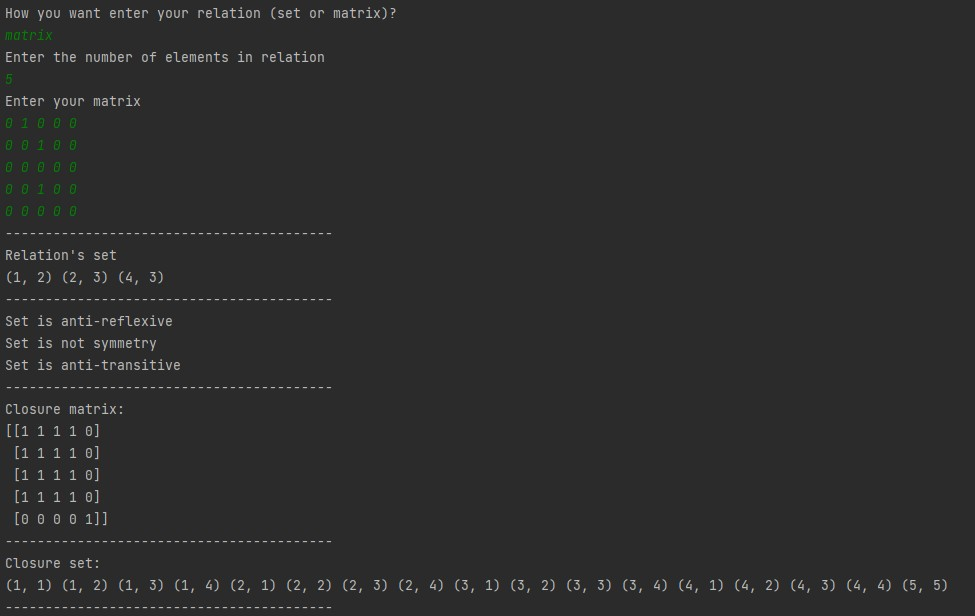
\includegraphics[width=1.\textwidth]{4}
            \caption{Тест 4}
            \label{fig:image1}
        \end{figure}

        \subsection{Оценки сложности рассмотренных алгоритмов}

        \subsubsection{Алгоритм определения рефлексивности}

            Сложность выполнения проверки на рефлексивность или антирефлексивность определяется как $O(n)$.

        \subsubsection{Алгоритм определения симметричности}

            Cложность транспонирования в numpy определяется как $O(n^{3/2}log \text{ } n)$, сложность умножения матриц 
            определяется как $O(n^3)$, сложность сравнение двух матриц поэлементно определяется как $O(n^2)$. 
            Отсюда можно сделать вывод, что в случае, если наше отношение будет симметричным,
            что будет являтся лучшим случаем раоты алгоритма,то общая сложность алгоритма будет определятся как 
            $O(n^{3/2}log \text{ } n + n^2) = O(n^{3/2}log \text{ } n)$,
            иначе, в худшем случае, сложность будет определятся как $O(n^{3/2}log \text{ } n + n^2 + n^2 + n^3) = O(n^3)$

        \subsubsection{Алгоритм определения транзитивности}

            Из всего выше сказанного очевидно, что сложность проверки на транзитивность или антитранзитивность составляет $O(n^3)$,
            так как в нем используется умножение, сравнение матриц и тройной цикл для проверки рефлексивности в худшем случае матриц.

        \subsubsection{Алгоритм классификации}
            Сложность выполнения самого алгоритма классификации бинарных отношений реализованно через питоновский словарь 
            и оператор if, поэтому является константной ($O(1)$), если не учитывать сложность выполнения проверки свойств отношения.

        \subsubsection{Построение замыкания рефлексивности}
        
            Так как весь алгоритм строится на заполнении главной диагонали матрицы 1, то его сложность состовляет $O(n)$.

        \subsubsection{Построение замыкания симметричности}

            Для посторения замыкания симметричности используются вложенный цикла, поэтому сложность алгоритма
            определяется как $O(n^2)$.

        \subsubsection{Построение замыкания транзитивности}

            Для посторения замыкания транзитивности используются два вложенный цикла, поэтому сложность алгоритма
            определяется как $O(n^3)$.
    
\conclusion

В рамках данной лабораторной работы были рассмотренны теоритические основы свойств бинарных отношений, их видов и методов
их замыкания по каждому из свойств. На основе этой теоретической части была смоделирована программа, которая способна
определить свойства заданного множества, его вид и построить систему замыкания по каждому из основных свойств бинарного
отношения.

\end{document}
